% vim: set spelllang=fr:
\chapter{Introduction}
\label{ch:intro}

\section{Motivation}

\subsection{Historique}

% TODO citer AIAMA plutôt
En Intelligence Artificielle et Traitement Automatique des Langues, les années
50 et 60 étaient pleines d'optimisme. D'après \citep{russell2010artificial},
Simon Herbert annonçait en 1957 :

\begin{quote}
    Mon intention n'est pas de vous surprendre ou de vous choquer, mais la
    manière la plus simple de résumer les choses consiste à dire qu'il existe
    désormais des machines capables de penser, d'apprendre et de créer. En
    outre, leur capacité d'accomplir ces choses va rapidement s'accroître
    jusqu'à que, dans un futur proche, le champ des problèmes qu'elles pourront
    aborder soit coextensif à celui auquel s'applique l'esprit humain.
\end{quote}

Effectivement, les réussites sur des petits problèmes étaient prometteuses.
\cite{slagle1963heuristic} a proposé un système de calcul de primitives du
niveau d'un bon étudiant de première année à l'université.
\cite{winograd1971procedures} a lui proposé un système de compréhension de
l'anglais au sein du monde des blocs, un micromonde très utilisé à l'époque
pour sa simplicité. Malheureusement, la réussite sur des petits problèmes ne
s'est pas étendue à des problèmes plus complexes, ce qui a conduit à un arrêt
des financements aux États-Unis \citep{pierce1966alpac} et à une forte
réduction en Grande Bretagne \citep{lighthill1973artificial}.

Depuis, l'Intelligence Artificielle a continué à progresser jusqu'à devenir une
industrie et une science, grâce à :
\begin{itemize}
    \item des techniques comme les systèmes experts, les réseaux de neurones et
        diverses approches d'apprentissage automatique,
    \item de gros volumes de données disponibles depuis le début des années
        2002,
    \item et à diverses applications tel que le filtrage des spams, la
        reconnaissance de la parole ou encore la robotique.
\end{itemize}

De la même manière, au fil des années, le Traitement Automatique des Langues a
muri, et s'appuie aujourd'hui sur des applications, des méthodes et des
sous-tâches plus accessibles que les applications envisagées initialement. Nous
citerons ici deux de ces sous-tâches.

\begin{itemize}
    \item \textbf{Étiquetage morpho-syntaxique} Le Brown Corpus a été annoté en
        parties du discours entre le milieu des années 60 et la fin des années
        1970, ce qui a permis d'entraîner divers algorithmes, tels que les
        chaînes de Markov cachées et plus tard des méthodes d'apprentissage
        supervisées telles que les SVMs ou les CRFs. Un plateau a été atteint
        autour de 97~\% d'exactitude depuis le milieu des années 2000
        \citep{manning2011part}.
    \item \textbf{Analyse syntaxique} Au début des années 1990, le corpus du
        Penn Treebank \citep{marcus1993building} a permis d'avancer la
        recherche en analyse syntaxique. Différents chercheurs ont introduit un
        certain nombre d'algorithmes ayant chacun leurs avantages et leurs
        défauts, la représentation en dépendances semble avoir été largement
        adoptée. Depuis le début des années 2010, et de la même manière que
        pour l'annotation des parties du discours, un plateau a été atteint
        autour de 90~\% d'exactitude, et ceci que la méthode soit statistique
        ou plus symbolique \citep{clergerie2014improving}.
\end{itemize}

Pour un certain nombre de chercheurs
\citep{bos2012annotating,banarescu2013abstract}, c'est le moment de se tourner
vers de nouvelles tâches plus sémantiques. C'est pour cette raison qu'à la
manière des corpus annotés en parties du discours ou en syntaxe qui ont tant
fait progresser leurs domaines respectifs, des corpus «~sémantiques~» ont vu le
jour dans le passé tels que FrameNet, PropBank ou RSTBank, mais d'autres, plus
ambitieux, voient aussi le jour aujourd'hui
\citep{bos2012annotating,banarescu2013abstract}
(section~\ref{ressources_non_utilisees}) dans le but affiché de «~faire
progresser la sémantique comme la syntaxe a progressé dans les années 1990~».

\subsection{Au-delà de l'analyse syntaxique}
\label{au_dela}

Dès lors, si l'on considère que l'analyse syntaxique n'est plus la priorité,
quelle direction prendre ? Commençons par identifier les informations
manquantes une fois que l'analyse syntaxique d'une phrase a été effectuée.

Le problème principal que nous voyons est que le sujet et les objets
syntaxiques d'un verbe ne suffisent pas à déterminer les sujets et objets
sémantiques, c'est-à-dire l'agent, le patient, etc. Par exemple, étant donné la
phrase \textit{Le ballon repoussé par Léa a cassé la vitre des voisins}, il
s'avère que le sujet syntaxique (\textit{Le ballon repoussé par Léa})
correspond parfaitement à l'agent sémantique.  Dans d'autres situations, ce
n'est pas le cas : pour \textit{La vitre des voisins a cassé sous le choc du
ballon tiré par Léo}, le sujet syntaxique est \textit{La vitre des
voisins}\footnote{Si la voix passive avait été employée, comme dans \textit{La
    vitre des voisins a été cassée par le choc du ballon tiré par Léo}, alors
le sujet syntaxique aurait bien été \textit{le choc du ballon tiré par Léo},
mais ce n'est pas le cas ici.}. Pourtant ce sujet syntaxique n'est pas l'agent
sémantique, mais bien le patient, étant donné que c'est la vitre qui subit
l'action ici.

De manière plus marquée que pour les sujets, l'analyse syntaxique en tant que
telle ne fournit pas suffisamment d'information pour désambiguïser le rôle des
objets du verbe.  Prenons les phrases \textit{Luc a posé un livre sur la table}
et \textit{Luc a posé sur la table son livre préféré traitant de la génétique des
chimpanzés}.  Ici, l'ordre des objets ne suffit pas, il faut identifier que
parmi les deux objets syntaxiques :

\begin{itemize}
    \item l'un est un syntagme prépositionnel introduit par une préposition
        locative (\textit{sur}),
    \item tandis que l'autre est un syntagme nominal direct.
\end{itemize}

On peut alors déterminer que le livre est le thème sémantique pour le prédicat
\textit{poser} et que la table est la destination sémantique pour ce même
prédicat. Ici, même si la syntaxe en elle-même ne résout pas le problème, c'est
bien grâce à elle qu'on peut déterminer le rôle de chaque syntagme.

Dans d'autres cas, la syntaxe ne suffit plus. Par exemple, pour la phrase
\textit{When you've booted the machine you've built yourself}, le sujet et
l'objet de \textit{boot} sont tous les deux des syntagmes nominaux, et la
syntaxe ne suffit alors pas à désambiguïser entre le sens informatique de
\textit{boot} (démarrer un ordinateur) et le sens géographique de \textit{boot}
(exclure un individu de quelque part). Ici, des informations sémantiques
peuvent nous aider. Dans le cas informatique, l'objet n'est pas animé, alors
que dans le second il l'est. Si on sait que \textit{the machine} n'est pas
animé. Il devient alors possible :

\begin{enumerate}
    \item d'exclure le sens géographique du verbe,
    \item et d'attribuer les rôles corrects aux syntagmes associés aux verbes
        (respectivement thème et destination),
\end{enumerate}

% C'est un peu tôt pour donner le lien entre frame-semantic parsing, WSD et
% SRL, mais où le mettre ?

Ces deux informations sont toutes les deux importantes : c'est bien le sens du
verbe qui permet d'interpréter les rôles sémantiques attribués aux syntagmes
dans une application.

Cette étape d'analyse au-delà de l'analyse syntaxique s'appelle l'annotation en
rôles sémantiques.

\section{Objectifs}

\subsection{L'annotation en rôles sémantiques}

L'annotation en rôles sémantiques répond à la question « Qui a fait Quoi à Qui,
Comment, Où et Quand ? ». Prenons pour exemple la phrase \textit{Mrs. Aouda
essaya vainement de retenir Mr. Fogg} (extrait du \textit{Tour du monde en
quatre-vingts jours} de Jules Verne). En considérant pour exemple le cadre de
FrameNet (section~\ref{presentation_framenet}), une annotation en rôles
sémantiques du prédicat \textit{essayer} déterminera que cette utilisation du
verbe correspond à une situation de Tentative, puis identifiera parmi les
syntagmes liés aux verbes quel est l'Agent, l'Activité tentée, et le Résultat.
Ainsi, le résultat de l'annotation serait :

\begin{figure}[ht]
    \centering
    \begin{tabular}{cccc}
    [Agent]  & \textbf{Tentative} & [Résultat]  & [Activité]         \tabularnewline
    Mrs. Aouda & \textbf{essaya}  & vainement & de retenir Mr. Fogg. \tabularnewline
    \end{tabular}
    \caption{\label{fig:introsrl}Le verbe \textit{essayer} déclenche la situation
        \textit{Tentative}. Les différents syntagmes liés au verbe jouent chacun
        un rôle sémantique ici, mais ce n'est pas toujours le cas. Par exemple,
        si la phrase précisait \textit{après le dîner}, ce syntagme aurait été un
    complément sans rôle sémantique associé.}

\end{figure}

Différentes informations sont disponibles après l'annotation en rôles
sémantiques :

\begin{itemize}
    \item Le prédicat ayant déclenché la situation est identifié. Dans la
        figure~\ref{fig:introsrl}, c'est un verbe. D'autres parties du discours
        peuvent déclencher une frame, mais nous nous concentrons dans ce
        travail essentiellement sur les verbes.
    \item La frame est identifiée, ici \textit{Tentative}.
    \item Enfin, les rôles exprimés sont annotés. Par exemple, \textit{Mrs.
        Aouda} est l'Agent.
\end{itemize}

\subsection{Applications}

Selon \cite{gildea2002automatic}, l'annotation en rôles sémantiques est
historiquement une évolution naturelle de certains travaux sur l'extraction
d'information où les systèmes traitent des situations très spécifiques, par
exemple la détection de résultats d'évènements sportifs ou la détection
d'acquisitions d'entreprises dans des corpus journalistiques. À chaque nouveau
système d'extraction d'information dans un domaine différent, il est nécessaire
de redéfinir les différents patrons sémantiques et d'entraîner un nouveau
système sur de nouvelles données, et l'annotation en rôles sémantiques est vue
comme une solution à ce problème. C'est dans cette optique que
\citeauthor{gildea2002automatic} s'appuient sur le corpus FrameNet et présentent le
premier système d'annotation en rôles sémantiques.

Aujourd'hui, les systèmes d'annotation en rôles sémantiques n'ont pas remplacé
les systèmes d'extraction d'information. Une des raisons est que les
difficultés sont différentes \citep{boros2014etiquetage} :

\begin{itemize}
    \item un système d'extraction d'information pourra utiliser plusieurs
        phrases pour remplir un évènement alors que l'annotation en rôles
        sémantique annote encore les phrases indépendamment,
    \item l'extraction d'informations se concentre sur un petit nombre
        d'évènements et d'étiquettes au sein d'un même évènement alors que les
        systèmes d'annotations en rôles sémantiques doivent traiter un grand
        nombre de situations différentes, chacune ayant ses propres étiquettes.
\end{itemize}

L'annotation en rôles sémantiques a, par contre, été utilisée dans un grand
nombre d'autres applications, notamment les systèmes de questions-réponses
\citep{shen2007using}, l'extraction d'évènements \citep{exner2011using}, la
fouille d'opinion \citep{das2012structure} ou la traduction automatique
\citep{bazrafshan2013semantic,bazrafshan2014comparing}. Un des intérêts de la
généralité de l'annotation en rôles sémantiques est de s'adapter facilement à
de nouvelles tâches. Ainsi, l'annotation en rôles sémantiques à aussi été
utilisée sur des tâches peut-être moins classiques : l'évaluation de la
traduction automatique \citep{lo2011meant,chuchunkov2014applying}, la détection
de plagiat \citep{osman2012improved}, la prédiction des cours de bourse
\citep{xie2013semantic}, la génération de scènes 3D \citep{chang2014learning},
la recommandation fondée sur le contenu \citep{de2014exploiting}, la détection
de comparaisons de produits \citep{kessler2013detection} ou l'interprétation de
recettes de cuisine \citep{malmaud2014cooking}.

\subsection{Contraintes}

Nous souhaitons que notre système d'annotation en rôles sémantiques puisse être
utilisé dans un environnement industriel dans lequel d'une part cette
annotation en rôles sémantiques fournit des informations utiles au
développement de tâches applicatives et d'autre part les domaines à couvrir ne
sont pas connus à l'avance. Les contraintes suivantes découlent de ces
prérequis.

\paragraph{Cadre ouvert} Se contenter de certaines situations dans un domaine
fermé n'est pas satisfaisant. Les inventaires de sens utilisés doivent couvrir
au maximum les différents sens des mots d'une langue.

\paragraph{Langue française} Le français dispose encore d'un nombre limité de
ressources sémantiques en cadre ouvert, même si cet écart est en train de se
combler rapidement. En effet, au-delà des ressources développées dans les
années 1970 que nous présenterons à la section~\ref{sec:lvflg}, des progrès
récents laissent entrevoir un futur brillant. Le projet ANR ASFALDA
\citep{candito2014developing} produit un FrameNet annoté du français de grande
qualité mais avec une couverture encore limitée, et WOLF \citep{citewolf} est
une traduction automatique de WordNet \citep{fellbaum1998wordnet} qui a
progressé à la fois en précision et en couverture au fil des ans. Pour rester
dans un cadre ouvert, le système présenté doit pouvoir se contenter de
transpositions automatiques de ces ressources vers le
français.\footnote{L'exception ici est VerbNet, ressource traduite
    «~semi-manuellement~» vers le français (Chapitre~\ref{ch:verbnet}) mais qui
n'est encore ni finalisée ni homogénéisée.}. Avec cette approche de
mutualisation des ressources au niveau de la langue, chaque nouvelle
utilisation d'une de nos ressources est l'occasion de l'améliorer à la fois
pour utilisation immédiate mais aussi pour les utilisations futures.

\paragraph{Simplicité} Nous voulons que notre système soit très simple à mettre
en place et qu'il soit tout aussi facile de corriger quelques erreurs
spécifiques, même au prix d'une performance moins bonne que des approches plus
complexes dans le cas général. La stratégie que nous adoptons est de simplifier
nos systèmes afin que toute intervention manuelle sur les ressources soit
possible, puis de les améliorer une fois qu'ils ont montré leurs limites.

\paragraph{Efficacité} Cette contrainte est moins forte que les autres, mais
reste nécessaire pour que les systèmes présentées puissent être utilisées à
large échelle. L'annotation en rôles sémantiques est un problème difficile de
classification automatique et certains systèmes ont des temps d'entraînement et
d'exécution trop longs pour l'utilisation que nous voulons en faire ici.

\paragraph{Libre diffusion} Enfin, il est important que les outils et
ressources soient au maximums libre d'accès afin que d'autres puissent les
utiliser et les étudier. Pour cette raison, la grande majorité du code source
écrit pendant cette thèse est disponible sur GitHub : en particulier, le
système d'annotation en rôles sémantiques est disponible sur
\url{https://github.com/aymara/knowledgesrl}. Il est utilisable indépendamment
mais a aussi été intégré dans l'analyseur linguistique libre LIMA
(\url{http://aymara.github.io/lima/}).

% MEGATODO faire que ce soit le cas
Ces contraintes seront utilisées pour évaluer à la fois l'état de l'art et les
approches présentées.

\subsection{Moyens}
\label{objectifs_these}

% TAL a besoin d'infos sur les verbes, c'est difficile et fragile, et on a
% besoin d'énormes corpus, donc on essaie les lexiques

Le Traitement Automatique des Langues requiert des lexiques et de larges
quantités de données annotées pour analyser efficacement des textes dans le
domaine général. Obtenir cette quantité de données est un problème en soi connu
sous le nom de "knowledge acquisition bottleneck" en désambiguïsation lexicale
\citep{gale1992method,navigli2009word}. Le problème se pose aussi pour
l'annotation en rôles sémantiques où la quantité de données annotées est
limitée \citep[section 1]{das2012structure}. Il est possible de résoudre ce
problème domaine par domaine en annotant de grandes quantités de données pour
chaque domaine, mais d'autres stratégies sont nécessaires pour mieux
généraliser et atteindre nos objectifs dans un grand nombre de domaines. Une
possibilité est d'utiliser au mieux les données annotées en perfectionnant les
algorithmes existants, une autre est d'utiliser intelligemment les données non
annotées qui existent en quantité bien plus importante. Une troisième
possibilité, celle que nous choisissons d'explorer ici, est d'exploiter des
lexiques couvrant l'interface syntaxe-sémantique sur une large partie du
vocabulaire. C'est ce qui est fait dans VerbNet où les traits syntaxiques et
sémantiques partagés par les mêmes verbes sont explicitement notés, ce qui
permet à chaque modification dans VerbNet d'améliorer le traitement de
plusieurs verbes au lieu d'un seul.

% VerbNet a montré son efficacité dans le domaine de par son approche
% pragmatique. Vient des classes de Levin, donne des correspondances entre
% syntaxe et sémantique

Deux difficultés majeures qu'affrontent les créateurs de lexique sont la
granularité de sens et la distinction des sens. Ces deux difficultés sont
traitées par les classes de Levin \citep{levin1993english} qui sont à l'origine
de VerbNet. Dans ces classes, les verbes sont classifiés principalement à
travers leur alternances syntaxiques, ce qui fournit un critère qui est à la
fois facilement observable et qui produit des distinctions sémantiques
intéressantes (section~\ref{presentation_levin}) validées par des expériences
empiriques impliquant un grand nombre d'annotateurs
\citep{hartshorne2014verbcorner}.  VerbNet \citep{kipperschuler2005verbnet},
basé sur les classes de Levin, encode non plus les alternances mais les cadres
de sous-catégorisation valables pour chaque classe, et rajoute des informations
de rôle et de sémantique à travers une logique des prédicats simplifiée. De
nouvelles classes, constructions et verbes ont étés ajoutés à VerbNet au fil
des ans. Au-delà de son encodage efficace, VerbNet est un lexique adapté à la
tâche d'annotation en rôles sémantiques : on peut utiliser un cadre de
sous-catégorisation pour associer des syntagmes à des rôles thématiques
\citep{swier2005exploiting,pradet2013revisiting}. Grâce à sa couverture élevée
(plus de quatre mille verbes distincts) et son groupement de verbes utile,
VerbNet est bien adapté à l'annotation en rôles sémantiques.

% De la même manière, WordNet est complémentaire à VerbNet

WordNet \citep{fellbaum1998wordnet} est une autre ressource qui complète
VerbNet d'au moins deux façons.

\begin{itemize}
    \item D'une part, WordNet peut être utilisé pour désambiguïser le sens des
        verbes et donc aider à choisir la bonne classe VerbNet.
    \item D'autre part, comme indiqué à la section~\ref{au_dela}, certaines
        propriétés sémantiques des syntagmes (animé, humain, organisation,
        etc.) sont utiles à l'annotation en rôles sémantiques, et la hiérarchie
        offerte par WordNet est le moyen idéal pour déterminer ces propriétés
        (section~\ref{restrictions_selection}).
\end{itemize}

% Dans les langues autres que l'anglais, cette ressource utile n'existe pas
% mais ne demande qu'à exister étant donné le potentiel \textit{cross-lingual}
% de VerbNet. Il y a souvent des ressources proches, moins utiles, plus
% linguistiques, existent.
Cependant, un VerbNet et un WordNet validés manuellement et à large couverture
n'existent pour le moment que pour l'anglais\footnote{L'exception est plWordnet
\citep{maziarz2012approaching}, un wordnet du polonais de grande taille validé
manuellement et toujours développé activement}. De telles ressources seraient
pourtant encore plus utiles pour les langues moins dotées où les corpus annotés
en rôles sémantiques n'existent pas.  VerbNet a un potentiel
inter-linguistique, visible notamment avec le portuguais \citep[section
2.2.2]{kipperschuler2005verbnet}. Adapter VerbNet vers une nouvelle langue
suffisamment proche de l'anglais permet de conserver sa structure, ainsi que
l'information sémantique et les rôles thématiques, ce qui donne la possibilité
de produire un lexique utile en économisant beaucoup de travail manuel.

Une fois que ces ressources ont été traduites vers le français, il faut les
utiliser pour réaliser la tâche d'annotation en rôles sémantiques. Cette thèse
fournit les \textit{ressources} nécessaires en traduisant WordNet et VerbNet
(Partie~\ref{part:translation}) et les \textit{méthodes} (Partie~\ref{part:srl})
répondant à ces objectifs.

\section{Ressources lexicales utilisées}
\label{ressources_utilisees}

\subsection{WordNet}
\label{presentation_wordnet}

La première ressource lexicale à tirer parti de la possibilité de représenter
le lexique sous la forme d'un graphe est WordNet \citep{fellbaum1998wordnet}.
Son élaboration a commencé en 1985 \citep{miller1990introduction}. Établi sur
des principes psycholinguistiques, WordNet propose quatre graphes pour les
quatre parties du discours formant une classe ouverte : noms, verbes,
adjectifs et adverbes. Les nœuds du graphe sont des ensembles de synonymes
(\textit{synonym sets} ou \textit{synsets}). Un synset regroupe plusieurs mots, une
définition, et potentiellement des exemples.

\begin{figure}[t]
    \centering
    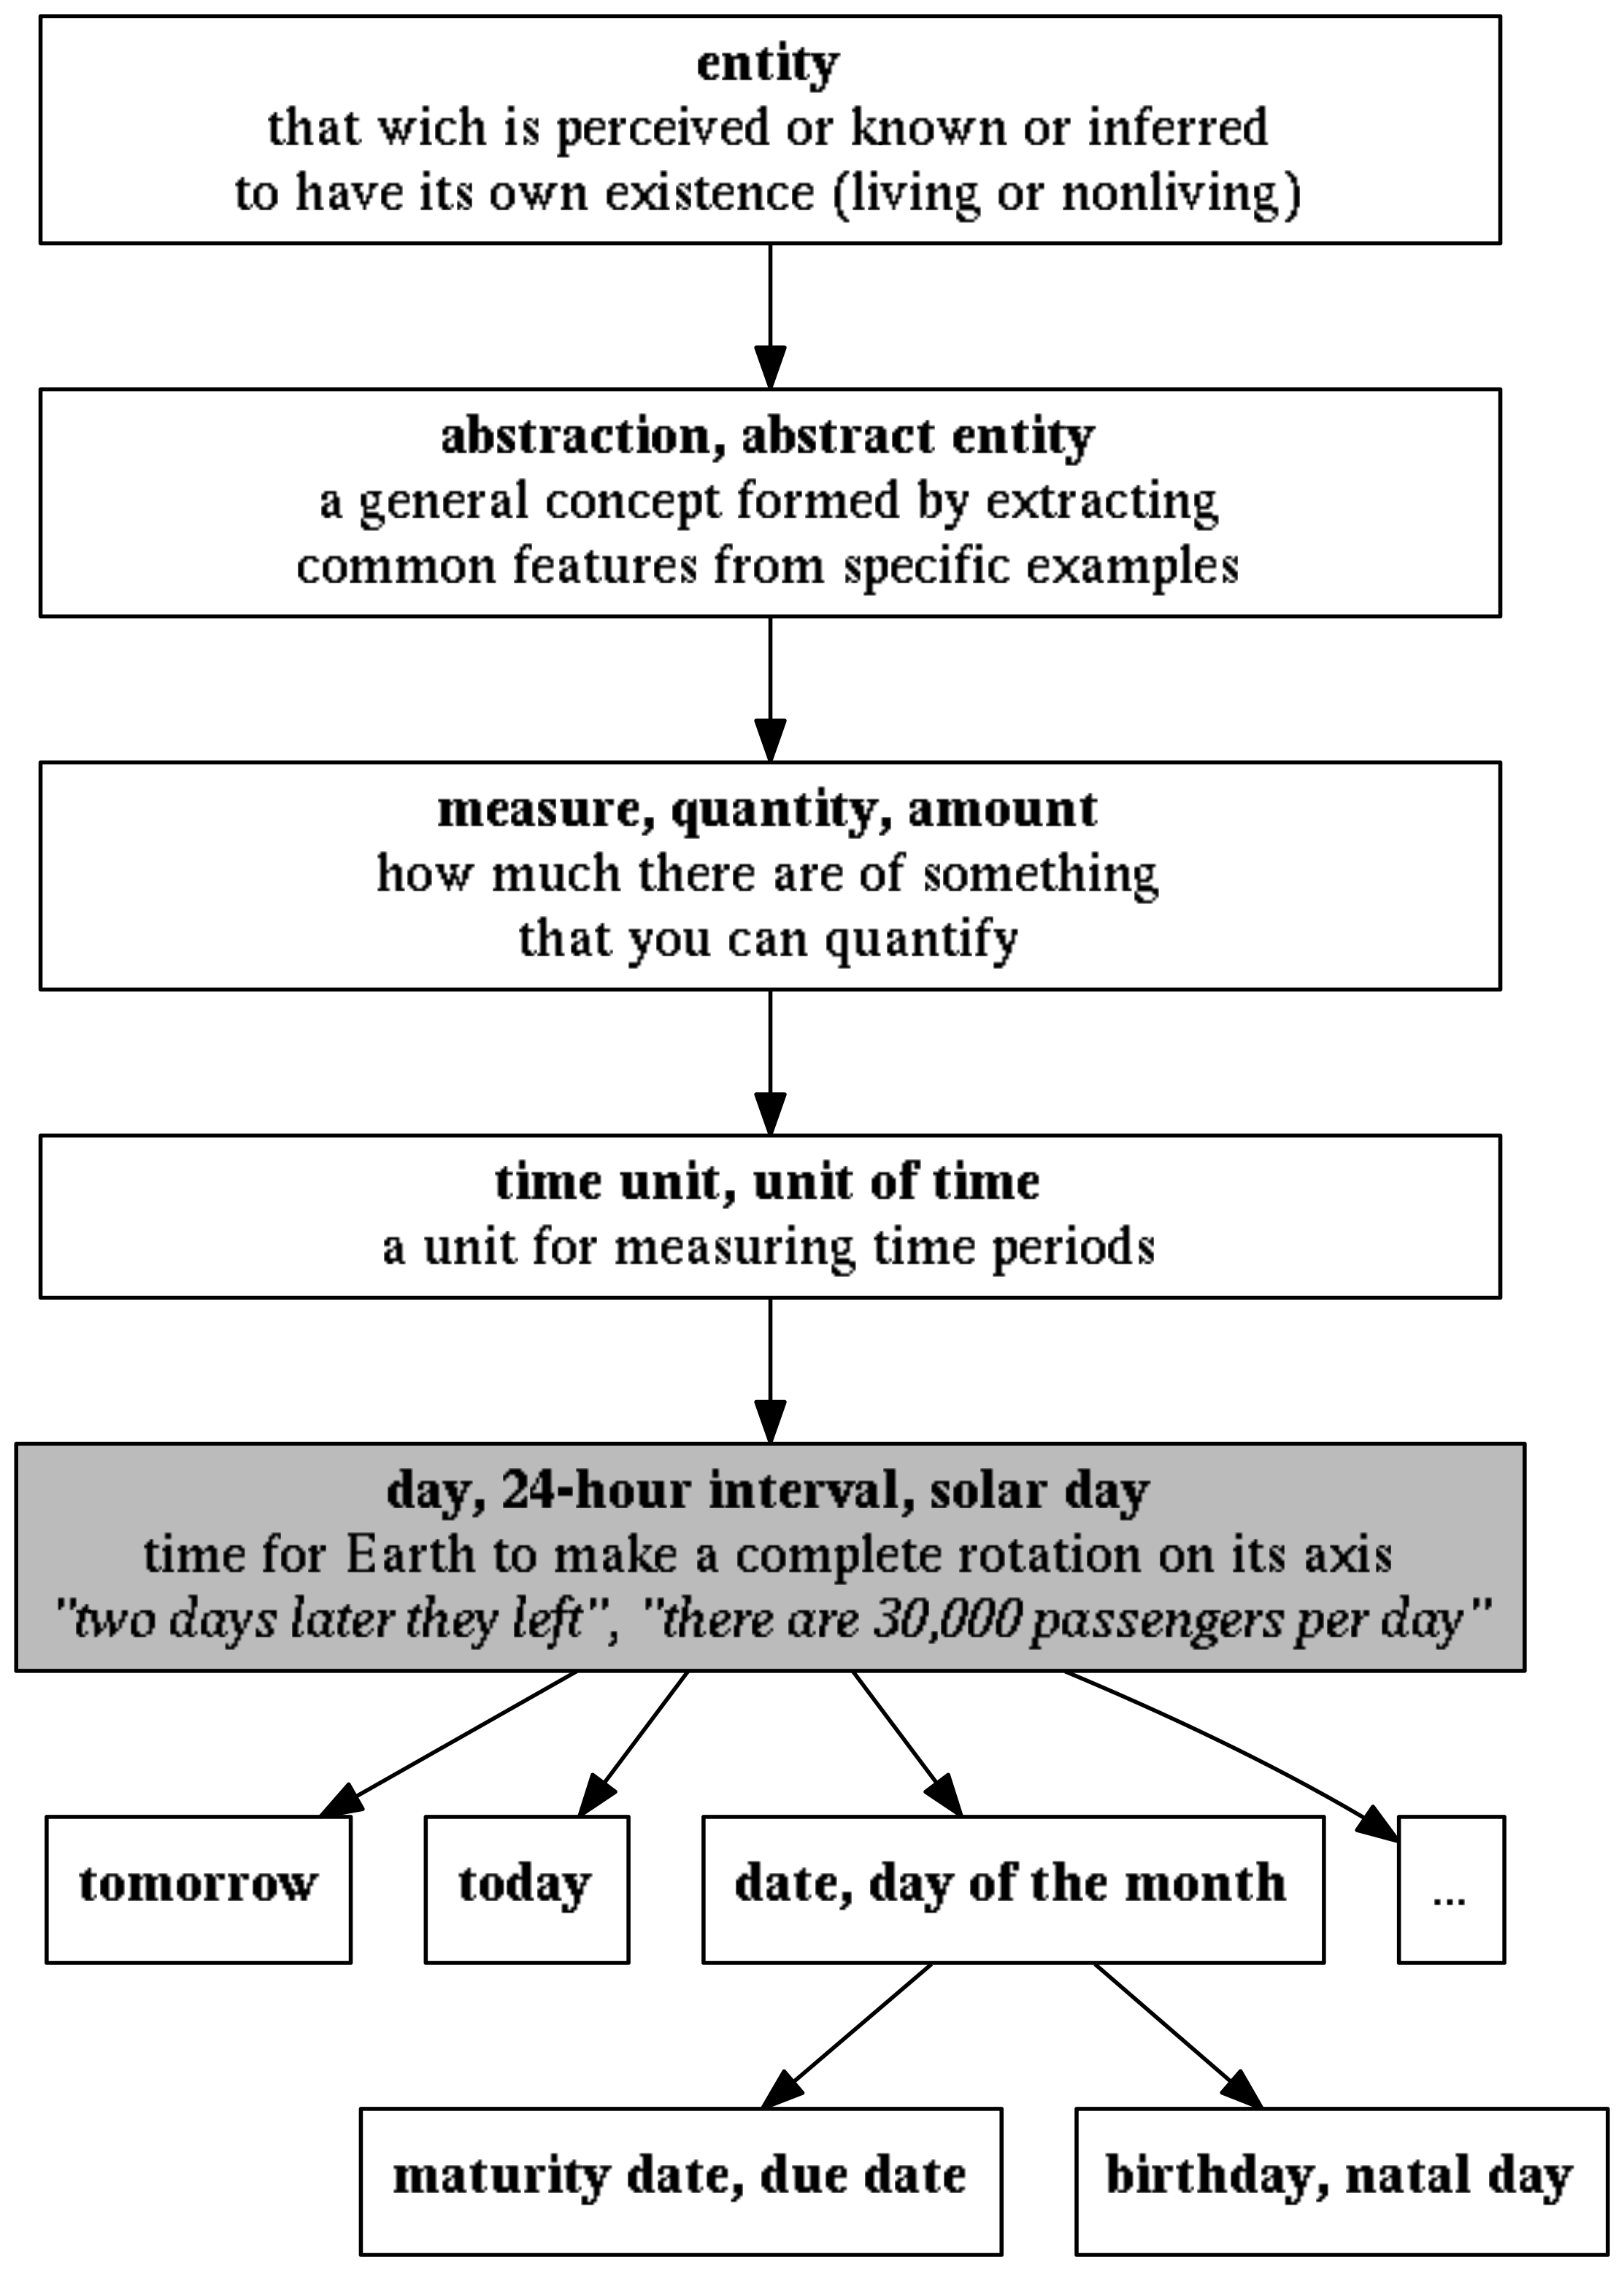
\includegraphics[width=0.6\textwidth]{fig/wordnet_hypernymy.png}
    \caption{\label{fig:wordnet_hypernymy}Hypéronymie dans WordNet autour du
        synset \textit{day}. Les synsets au-dessus de \textit{day} sont ses hypéronymes
        (\textit{day} est-un \textit{time unit}), et les synsets au-dessus font partie de
        ses hyponymes (\textit{tomorrow} est-un \textit{day}).}
\end{figure}

Chaque synset est lié à d'autres synsets à travers un certain nombre de
relations telles que l'hypéronymie, la méronymie de partie (\textit{guidon} est
un méronyme de partie de \textit{vélo}), l'antonymie, etc. Si on ne considère que
l'hypéronymie, WordNet peut être visualisé comme un arbre
(Figure~\ref{fig:wordnet_hypernymy}). En considérant les autres relations,
WordNet est un graphe (Figure~\ref{fig:wordnet_relations}).

\begin{figure}
    \centering
    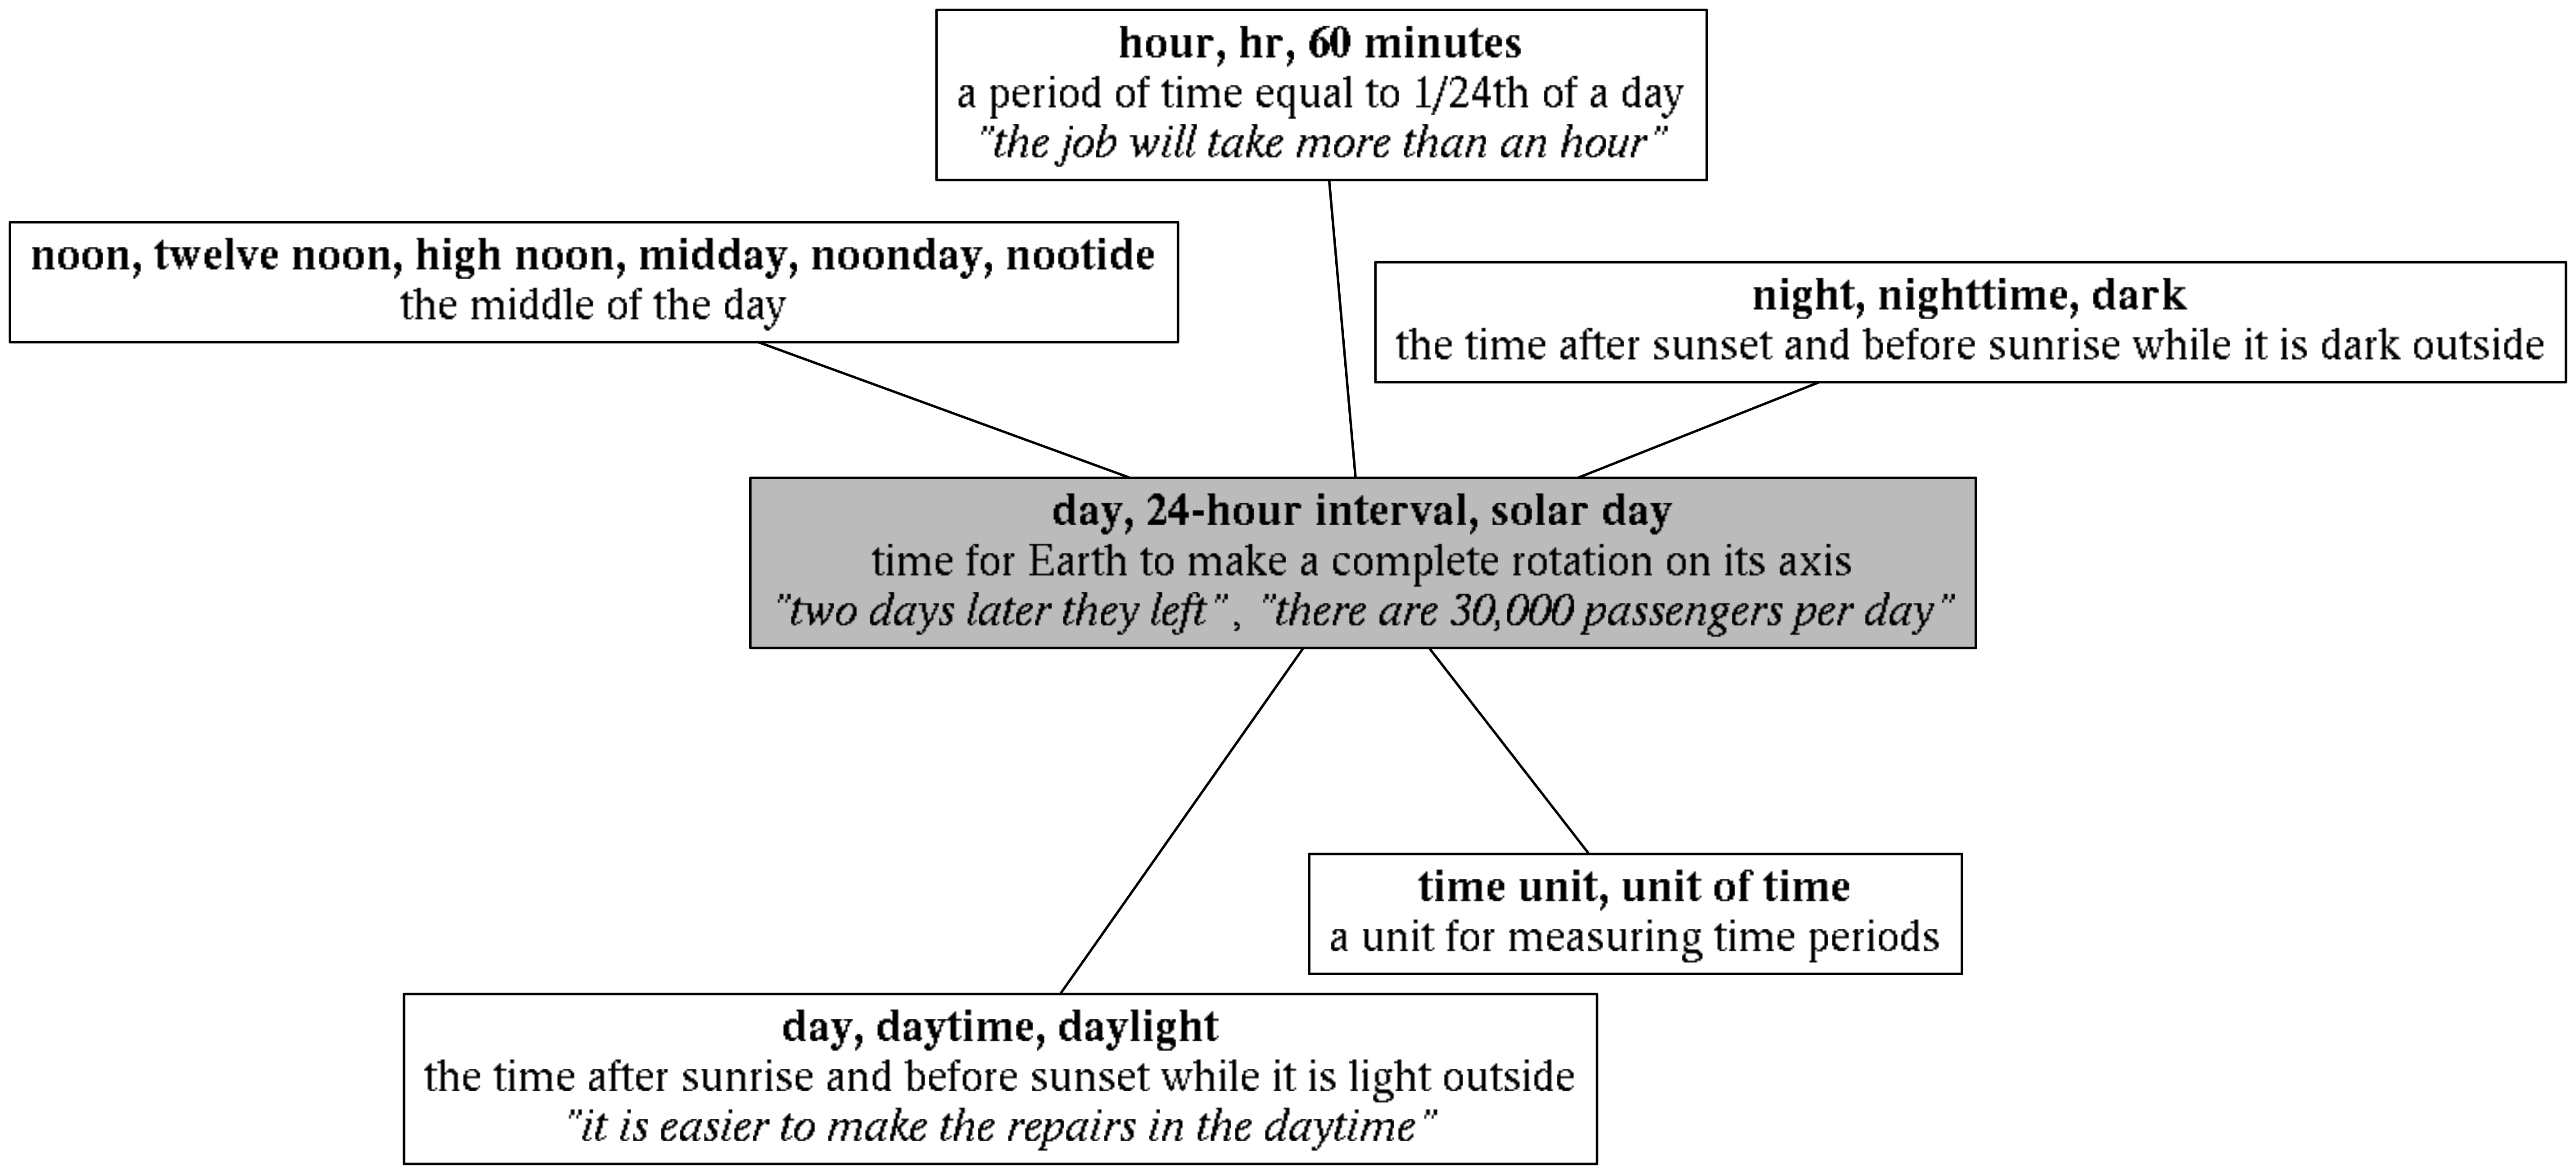
\includegraphics[width=\textwidth]{fig/wordnet_relations.png}
    \caption{\label{fig:wordnet_relations} Le synset \textit{day} est aussi lié à
        d'autres synsets si on considère d'autres relations que l'hypéronymie et
        l'hyponymie.}
\end{figure}

Les sens proposés par WordNet ont étés utilisés pour annoter différents corpus
\citep{petrolito2014survey}, ce qui a permis d'entraîner des systèmes
supervisés. WordNet est rapidement devenu le standard de la désambiguïsation
lexicale et a été utilisé dans de nombreuses campagnes d'évaluation
\citep{navigli2009word}. C'est aussi une ressource très utilisée pour beaucoup
d'applications : au moment de l'écriture de ce manuscrit, ses 10~000 citations
sur Google Scholar sont le meilleur moyen de l'attester.

\subsection{Les classes de Levin}
\label{presentation_levin}

Les classes de Levin \citep{levin1993english} sont une classification des
verbes anglais établie suivant un principe simple : le comportement syntaxique
des verbes détermine en partie leur sens. Après avoir défini un certain nombre
d'alternances de diathèses possibles, les verbes sont classés en groupes
partageant les mêmes alternances.

Par exemple, les \textit{fill verbs} tels que \textit{staff}, \textit{coat} ou encore
\textit{pollute} \citep[p.~119]{levin1993english} acceptent notamment la
\textit{locatum subject alternation} \citep[p.~85]{levin1993english}, donc ces
deux constructions sont possibles :

\begin{itemize}
    \item \textit{Leslie staffed the store with employees}
    \item \textit{The employees staffed the store}
\end{itemize}

mais n'acceptent pas par exemple, la \textit{conative alternation}
\citep[p.~41]{levin1993english}, donc seule la première construction est
possible :

\begin{itemize}
    \item ~ \textit{Leslie staffed the store with employees}
    \item * \textit{The store staffed with employees}
\end{itemize}

Ainsi, pour chaque groupe de verbes, différents critères précis permettent de
distinguer ces verbes d'autres qui n'ont pas les mêmes propriétés.

Cette classification a trois intérêts pour l'annotation en rôles sémantiques :

\begin{itemize}

    \item Une grande majorité des verbes anglais sont couverts, rendant la
    ressource utile pour des annotations à large échelle.

    \item La classification est hiérarchique et regroupe de nombreux verbes :
    avec une cinquantaine de classes principales, des généralisations et
    partages d'informations entre les verbes de classes identiques ou proches
    sont possibles.

    \item Les comportements syntaxiques déterminent les comportements
    sémantiques, ce qui correspond au schéma classique de l'annotation en rôles
    sémantiques qui s'appuie avant tout sur une analyse syntaxique.

\end{itemize}

Dans les classes de Levin, toute distinction de classe doit s'appuyer sur un
critère clairement observable, tel que le comportement syntaxique ou les
propriétés morphologiques d'un verbe. Ainsi, même dans les cas où l'on veut
identifier une différence sémantique provenant d'une intuition linguistique, il
faut établir des critères clairs et précis permettant d'assurer la cohérence et
la robustesse de l'ensemble.

Pour cette raison, les groupements de verbes sont parfois grossiers d'un point
de vue sémantique. Ainsi, dans les \textit{put verbs} se trouve la classe
\textit{Pocket} qui regroupe les verbes "mettre dans sa poche" (\textit{put}) et
"mettre en prison" (\textit{jail}). Cependant, le comportement syntaxique est le
même : le regroupement est logique et les différences de sens ne sont a priori
pas gênantes pour des tâches telles que l'annotation en rôles sémantiques qui
ne se basent pas sur le sens précis des verbes. Si ce manque de finesse est
gênant, il est possible d'affiner automatiquement les classes de Levin en
réalisant des intersections de classes : les verbes obtenus seront alors
définis plus strictement \citep{dang1998investigating}. Cette possibilité n'est
cependant pas utilisée dans nos travaux.

\subsection{VerbNet}
\label{presentation_verbnet}

\begin{figure}[p]
    \centering
    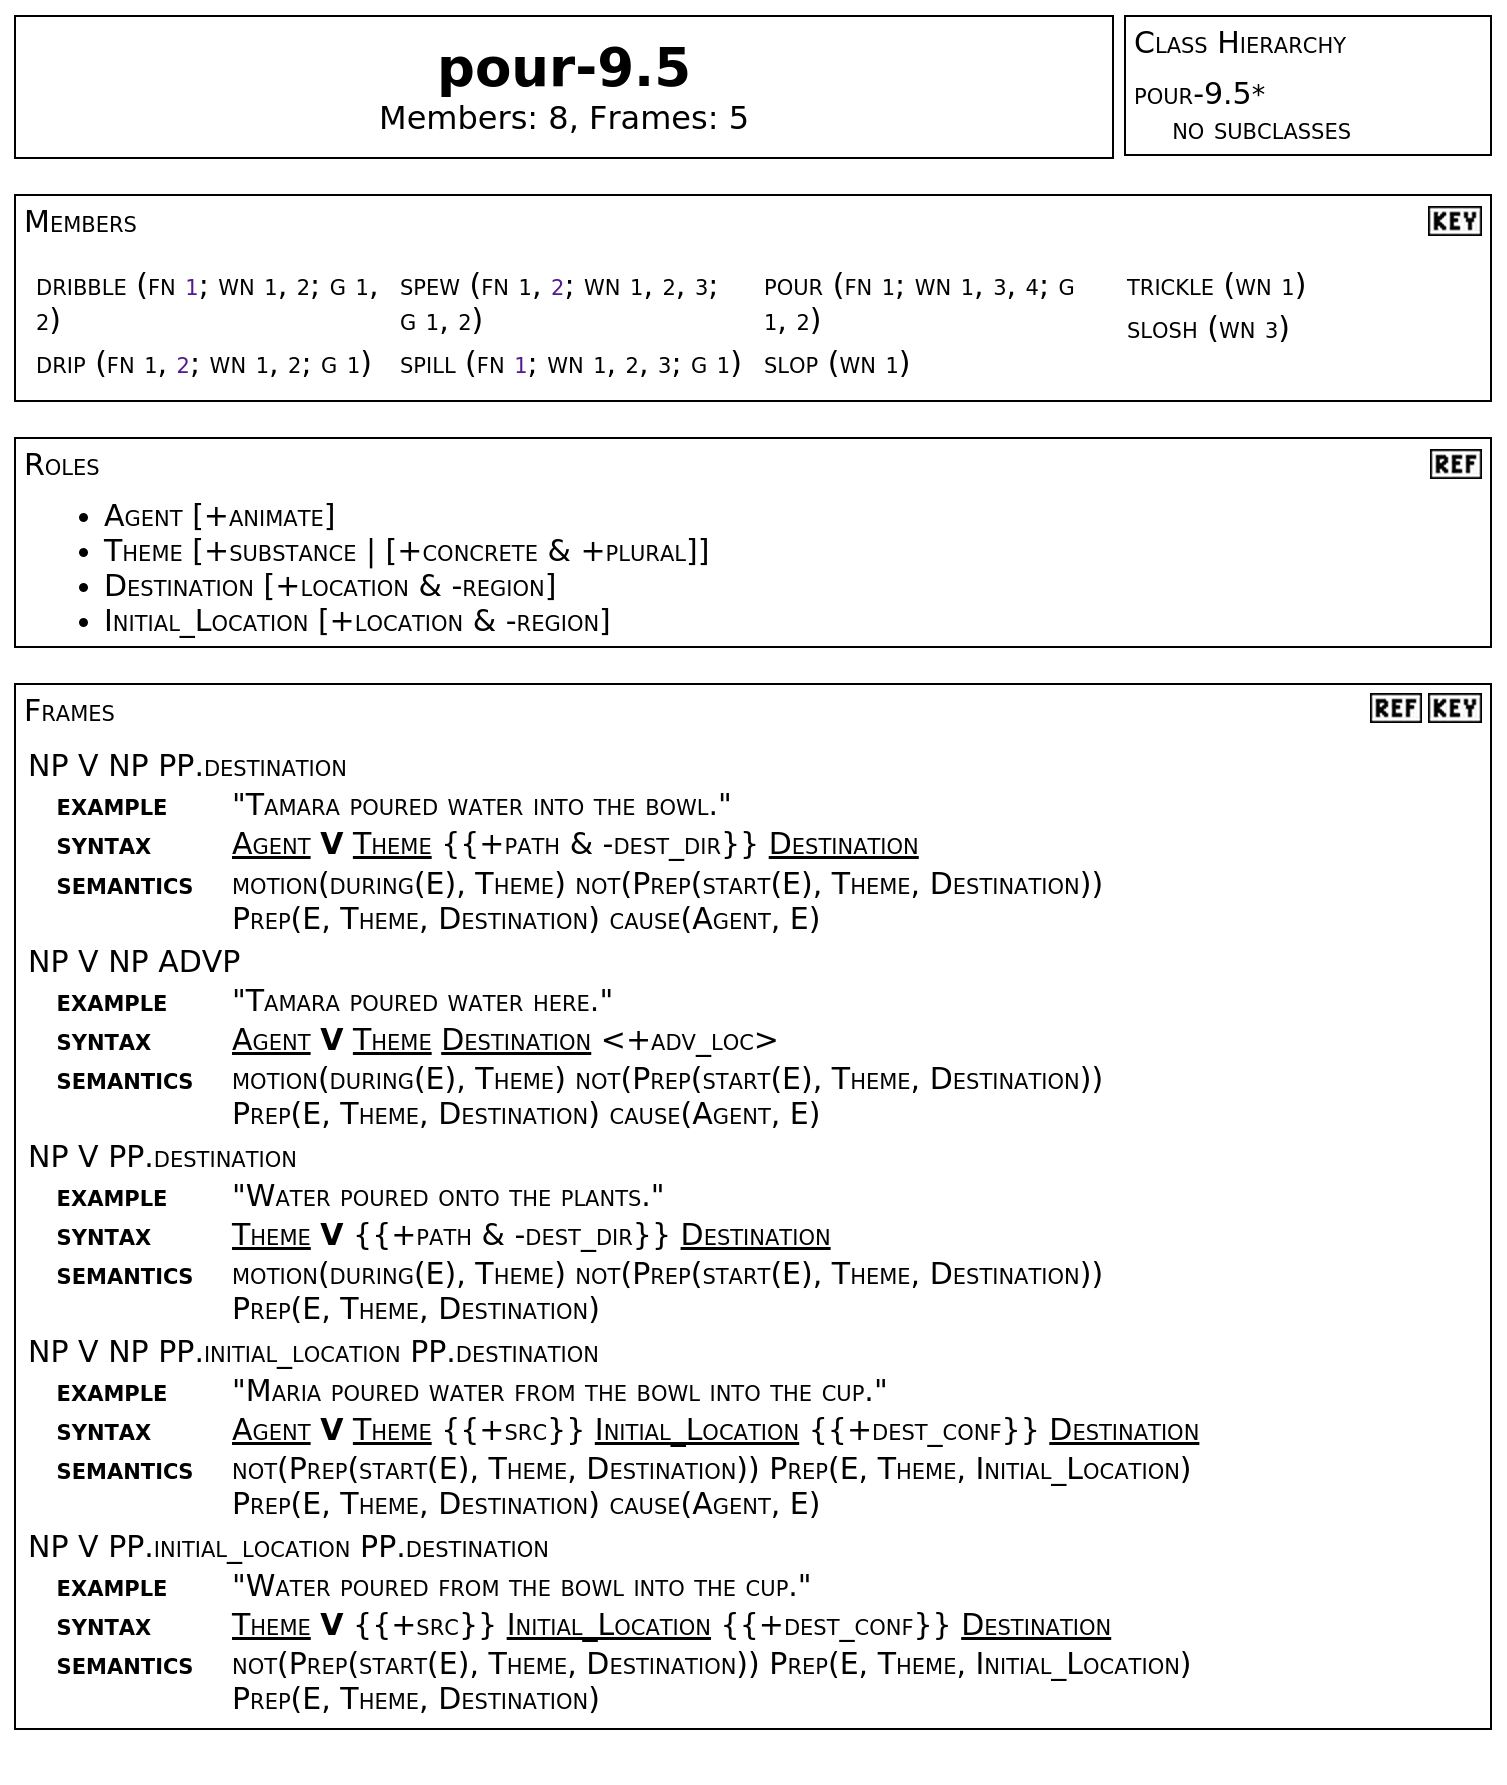
\includegraphics[width=\textwidth]{fig/verbnet_pour_class.png}
    \caption{\label{fig:exemple_verbnet}La classe \texttt{pour-9.5} dans
    VerbNet. Huit membres sont listés avec des mappings vers FrameNet (FN),
    WordNet (WN) et les groupements OntoNotes (G). Les rôles sont associés à
    des restrictions de sélections : ici l'Agent est toujours animé. Les frames
    listent les constructions syntaxiques valides, avec un exemple et une
    interprétation sémantique. Cette classe n'a pas de sous-classes, mais si
    elle en avait, les frames de cette classes seraient valides pour les verbes
    de la sous-classe.}
\end{figure}

VerbNet \citep{kipperschuler2005verbnet} est une version électronique des
classes de Levin qui ont été améliorées sur plusieurs fronts avec :

\begin{itemize}

    \item de nouvelles classes provenant de \cite{korhonen2004extended}
        intégrant les verbes acceptant des complétives, mais aussi des
        syntagmes adjectivaux et adverbiaux ou encore des particules,

    \item de nouveaux verbes provenant de \cite{dorr2001lcs},

    \item la liaisons des verbes à WordNet, OntoNotes, PropBank et FrameNet
        dans le cadre du projet SemLink \citep{palmer2009semlink},

    \item de nombreuses corrections au fil des versions, une des améliorations
        prévues dans le futur étant d'ajouter d'autres verbes via l'étude de
        large corpus \citep{bonial2013expanding}.

\end{itemize}

Ces améliorations ont à la fois contribué à VerbNet en largeur (nouvelles
classes) et en profondeur (nouveaux verbes, nouvelles constructions
syntaxiques). La base de données continue d'évoluer, la dernière version au
moment de l'écriture de ce manuscrit étant la 3.2. Malheureusement, la version
3.2 évolue sans que soient marqués clairement les sous-versions : suivant le
jour de téléchargement de VerbNet, nous pouvons avoir à disposition la version
3.2.1, 3.2.2 ou 3.2.3, sans pouvoir clairement distinguer ces trois versions.
De plus, nous avons du modifier la ressource pour corriger certaines
incohérences que nous espérons voir incluses dans la prochaine version de
VerbNet. Pour cette raison, nous rendons disponibles la version de VerbNet que
nous utilisons dans l'ensemble de ce travail à l'adresse suivante :
\url{https://github.com/aymara/verbnet/archive/pradet-thesis.zip}.

VerbNet contient 3769 lemmes, 5257 entrées réparties en 500 sous-classes dont
270 classes de niveau 2 et 109 classes de niveau 1. Pour chaque sous-classe, ce
lexique indique :

\begin{itemize}
        \item la liste des verbes de la classe,
        \item les rôles thématiques en jeu ainsi que leur restrictions de sélection,
        \item la liste des \textit{frames} VerbNet,
        \item les éventuelles sous-classes.
\end{itemize}

Une frame inclut une phrase d'exemple, une formule syntaxique donnant la
liaison entre les syntagmes et les rôles thématiques, une formule sémantique
basée sur la logique des prédicats explicitant la relation entre les
participants et les évènements. La figure \ref{fig:exemple_verbnet} montre ces
différentes informations telles qu'elles sont listées sur le site web de
VerbNet pour la classe \texttt{pour-9.5} (disponible sur
\url{http://verbs.colorado.edu/verb-index/index.php}.


VerbNet a montré la cohérence de sa classification et est très utilisé,
notamment pour l'annotation en rôles sémantiques
\citep{swier2005exploiting,palmer2013semantic} où il présente l'intérêt de ne
pas être restreint à un domaine spécifique tout en couvrant une large partie
des occurrences des verbes anglais dans un texte donné.


\subsection{Les Verbes Français et Lexique-Grammaire}
\label{sec:lvflg}

À partir des années 1970 deux ressources lexicales pour les verbes français ont
été dévelopées : LVF et LG\footnote{Plus tard, dans les années 1990, une autre
    ressource a été dévelopée : Dicovalence. Nous ne l'utilisons presque pas
dans nos travaux.}.

LVF (Les Verbes Français, \cite{dubois1997verbes}) contient environ 25000
entrées classées en quatre niveaux :

\begin{itemize}

    \item 14 classes génériques (par exemple \textit{E : Verbes de mouvement}),

    \item 54 sous-classes sémantico-syntaxiques (par exemple \textit{C1 :
        s'exprimer par un son, une parole}),

    \item 246 sous-classes syntaxiques (par exemple \textit{M3b : imprimer tel
        mouvement à quelquec chose} et

    \item 533 sous-types (par exemple \textit{R3b.2 : défaire l'opération
        faite}).

\end{itemize}

% TODO exemple

LG (Lexique-Grammaire, \cite{gross1975methodes,boons1976structure}) comporte
lui 14 000 entrées classifiées en 67 «~tables~», chaque table groupant des
verbes partageant la même propriété définitoire syntaxique et potentiellement
une sémantique similaire. Chaque colonne de la table encode des restrictions
supplémentaires s'appliquant à certains des verbes de la table.

% TODO exemple

Pourquoi ne pas utiliser ces ressources directement dans nos travaux ? Pour
plusieurs raisons :

\begin{itemize}
    \item LVF inclut de nombreux usages techniques : il y a en réalité
        \textit{trop} de verbes et de sens : nous voulons nous concentrer sur les
        verbes les plus fréquents, environ 5~000.
    \item LVF (et dans une moindre mesure, LG), incluent de nombreux emplois
        métaphoriques, ce qui nuit à la ressource : des usages tels que
        \textit{Il galopait dans son esprit que Marie allait venir} (extrait de
        LG) ne sont pas souhaitables. Certains usages métaphoriques peuvent
        certes être prise en compte dans VerbNet, mais ils n'y sont pas par
        défaut. En effet, \cite{brown2012semantic} proposent une analyse
        systématique des emplois métaphoriques de deux verbes représentatifs et
        montrent qu'utiliser VerbNet pour raisonner sur les emplois
        métaphoriques d'un texte est en partie possible au prix d'une complexité
        plus importante et de prédicats sémantiques moins précis.
    \item LG ignore presque complètement la sémantique : de nombreuses classes
        auraient pu être séparées plus utilement en considérant des différences
        sémantiques exprimées par ailleurs dans la syntaxe.
    \item LVF, au contraire, se base sur des critères difficiles à comprendre et
        manifestement subjectifs, au contraire de VerbNet et LG.
    \item Ni LVF ni LG n'encodent de rôles thématiques ni de formules
        sémantiques\footnote{Les notions de rôles thématiques et d'évènement
        n'étaient pas répandues dans les années 1970.}.
\end{itemize}

Ce sont les raisons principales pour laquelle nous voulons construire une
nouvelle ressource française, \verbenet{} (Chapitre~\ref{ch:verbnet}). Cette
ressource tire profit d'une part des ressources existantes pour le français
avec un encodage sémantique et syntaxique riche, et d'autre part de
l'information sémantique présente dans VerbNet pour l'anglais, une langue
proche du français. \verbenet{} peut être vu dans une certaine mesure comme une
réorganisation des classes LG, étant donné que les deux ressources sont
essentiellement basées sur des critères syntaxiques.

\section*{Conclusion}

Après avoir introduit le cadre de nos travaux et présenté les différentes
ressources que nous utilisons, le chapitre suivant présente l'état de l'art qui
est le socle sur lequel nos travaux s'appuient.
